\thispagestyle{plain}
\begin{center}
\Large\textbf{Growth of interface cracks on consecutive fibers: on the same or on the opposite sides?}\\
\vspace{10mm}
\normalsize Luca Di Stasio$^{1,2}$, Janis Varna$^{1}$ and Zoubir Ayadi$^{2}$\\
\vspace{5mm}
\normalsize $^{1}$Lule\aa\ University of Technology, University Campus, SE-97187 Lule\aa, Sweden\\
\normalsize $^{2}$Universit\'e de Lorraine, EEIGM, IJL, 6 Rue Bastien Lepage, F-54010 Nancy, France\\
\vspace{15mm}
\textbf{Abstract}\\
\end{center}

The growth of fiber/matrix interface cracks (debonds) located on consecutive fibers along the through-the-thickness (vertical) direction is studied in glass fiber-epoxy UD composites. Two different families of Representative Volume Elements (RVEs) are developed: the first implements the classic condition of coupling of the vertical displacements to model a unit cell repeating symmetrically along the vertical direction; the second uses a novel set of boundary conditions, proposed here by the authors, to represent a unit cell repeating anti-symmetrically along the vertical direction. The model is analyzed in the context of Linear Elastic Fracture Mechanics (LEFM) and the Mode I and Mode II Energy Release Rate are evaluated to investigate crack growth. The calculation is performed using the Virtual Crack Closure Technique (VCCT) in the framework of the Finite Element Method (FEM). It is found that Mode I dominated propagation is favored when debonds are located on the same sides of their respective fibers; while for larger Mode II-dominated debonds, Mode II ERR is higher when they lie on the opposite sides. No effect is present when at least two fully bonded fibers are located between the partially debonded ones.

\vspace{5mm}

\textbf{Keywords:} Polymer Matrix Composite (PMC), Transverse cracking, Debonding, Debond Interaction


%%%%%%%%%%%%%%%%%%%%%%%%%%%%%%%%%%%%%%%%%%%%%%%%%%%%%%%%%%%%%%%%%%%
% 1. INTRODUCTION
%%%%%%%%%%%%%%%%%%%%%%%%%%%%%%%%%%%%%%%%%%%%%%%%%%%%%%%%%%%%%%%%%%%

\section{Introduction}

Organized and completed over the last three decades, the three World Wide Failure Exercises (WWFEs)~\cite{Hinton2004,Hinton2012,Kaddour2013a} represent one of the most comprehensive attempts to date to evaluate the maturity of failure criteria and predictive theories of damage of Fiber-Reinforced Polymer Composites (FRPC). The third and last one (WWFE-III) aims at providing a benchmark for models of sub-critical damage, namely matrix cracking, delamination and fiber failure, by comparing the independent predictions of 12 different approaches (each one from a different individual, group or institution) over 13 test cases~\cite{Kaddour2013a}. The comparison of predictions by the different theories shows a wide scatter of results, symptomatic of the immaturity of the field~\cite{Kaddour2013b}. Furthermore, it uncovers the existence of gaps in the knowledge shared by all models. Among these, a clear understanding is still elusive regarding the mechanisms of initiation of an individual transverse crack.\\
Onset of transverse cracks is determined at the microscopic level by initiation and propagation of fiber-matrix interface cracks~\cite{Bailey1981,Bailey1979}, or debonds. Debonds first grow along the arc direction of the fiber; at a certain critical size they kink out of the interface and lead to the onset of matrix micro-cracks; micro-cracks coalesce together forming a through-the-thickness crack~\cite{Zhang1997}; this crack finally propagates along the fiber direction, i.e. “tunneling” across the width of the laminate, and creating a transverse crack. Thus, understanding the mechanism of debond growth and predicting debond critical arc size (at which kinking starts) represent an important step in the development of precise predictive models of transverse cracking.

\begin{figure}[!htb]
\centering
  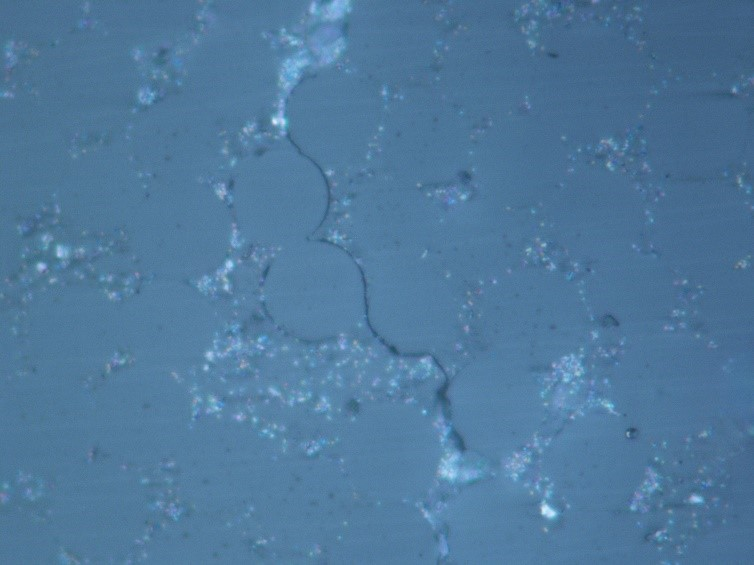
\includegraphics[height=0.225\textheight]{paperD/debonds.jpg}
\caption{Debonds in the $90^{\circ}$ layer of a $\left[0^{\circ}/90^{\circ}\right]_{S}$ laminate after being subjected to tensile strain in the horizontal direction.}\label{paperD:fig:debonds-microscope}
\end{figure}

Initial attempts to analyze the mechanics of debonding were based on the linear elastic solution of a single partially debonded fiber in an infinite matrix with an applied tensile stress at infinity, evaluated analytically by using complex potentials ~\cite{England1966,Perlman1967,Toya1974}. It was found that stress and displacement fields have an oscillating singularity at the crack tip, which prevents the use of Stress Intensity Factors (SIFs) as they are not defined at the debond tip. Similarly, Mode I and Mode II Energy Release Rate (ERR) do not converge and mode-based partition of the ERR is not possible. However, the ERR can be interpreted as the work needed to open the crack by an infinitesimal amount da or equivalently, in the case of Linear Elastic Fracture Mechanics, to close the crack by the same infinitesimal amount $da$. By considering a small but finite crack increase $\Delta a$ instead of the infinitesimal increase $da$, the lack of convergence due to the oscillatory singularity can be circumvented and an approximation of Mode I and Mode II ERR can be provided. The recurse to this strategy makes the problem suitable for a resolution technique based on domain discretization such as the Finite Element Method (FEM) or the Boundary Element Method (BEM). In subsequent works~\cite{Paris1996,Varna1997a}, it was shown that Toya’s analytical solution~\cite{Toya1974} implies a non-physical interpenetration zone in the crack tip neighborhood. This led to the introduction of a no-interpenetration contact interaction which, solved with the Boundary Element Method (BEM), showed the existence of a contact zone (a finite size region in which crack faces are in contact) for debonds larger than a critical value~\cite{Varna1997a}. In ~\cite{Garcia2015}, the authors compared the one-debond with respect to the two-symmetric-debonds configuration and found that the former is energetically the most favorable to crack growth. The effect of several load combinations on ERR of a single partially debonded fiber in an effectively infinite matrix was later studied~\cite{Correa2007,Correa2013,Correa2014}, as well as the effect of a neighboring fully bonded fiber~\cite{Sandino2016,Zhuang2018}. Researchers in~\cite{Varna2017} studied the effect on debond ERR of the presence of a second partially debonded fiber, with the two debonds placed facing each other (i.e. no fiber in between).\\
Microscopic observations of debond growth, such as the one reported in Fig.~\ref{paperD:fig:debonds-microscope}, show debonds developed on the same as well as the opposite sides of consecutive fibers on average aligned along the vertical, i.e. through-the thickness, direction. It is thus interesting to investigate the effect on debond ERR of the position of the next debond on the neighboring partially debonded fiber along the vertical direction. To this end, we develop Representative Volume Elements (RVEs) which, by application of displacement-coupling boundary conditions along the right and left sides, are repeating in a mirror-like fashion horizontally. The use of coupling conditions on the vertical displacement along the upper boundary models the presence of another partially debonded fiber with a debond of equal size and on the same side. In order to model the case of a fiber with a debond of equal size but appearing on the opposite side, we propose a set of anti-symmetric coupling conditions that are applied to the upper boundary. Details regarding coupling conditions, RVEs and Finite Element (FE) discretization are presented in Sec. \ref{paperD:sec:RVEs} and Sec. 3, while results are presented and discussed in Sec. 4.

%%%%%%%%%%%%%%%%%%%%%%%%%%%%%%%%%%%%%%%%%%%%%%%%%%%%%%%%%%%%%%%%%%%
% 2. RVE MODELS AND FE DISCRETIZATION
%%%%%%%%%%%%%%%%%%%%%%%%%%%%%%%%%%%%%%%%%%%%%%%%%%%%%%%%%%%%%%%%%%%

\section{Representative Volume Elements (RVEs)}\label{paperD:sec:RVEs}

Two families of RVE are studied in the present work. RVEs from both families:
\begin{itemize}
\item represent a Uni-Directional (UD) composite, infinite in all 3 directions (length, width and thickness);
\item are solved using plain strain conditions, and thus represent a debond whose length along the fiber is much greater than its arc size;
\item consider two linear, homogeneous, isotropic elastic phases, i.e. glass fiber and epoxy matrix, whose properties are reported in Table \ref{paperD:tab:phaseprop};
\item possess a centrally placed partially debonded fiber and have a total of $n$ fibers along the horizontal direction (loading direction, transverse to composite $0^{\circ}$ direction) and $k$ in the vertical (i.e. through-the-thickness) direction;
\item repeat infinitely along the horizontal direction in a mirror-like way (the next RVE to the right is the mirror image with respect to the right-side boundary) thanks to the application of coupling conditions on the horizontal displacement along the right and left sides of the element;
\item are symmetric with respect to the horizontal axis, which allows the discretization of only half RVE through the application of symmetry boundary conditions on the lower side;
\item are subject to tensile loading in the form of applied displacement corresponding to a $x$-strain level of $1\%$.
\end{itemize}
The distinction between the two families of RVE lies in the boundary conditions applied along the upper side.

\begin{table}[!htbp]
 \centering
 \caption{Material properties of glass fiber and epoxy adopted in the present study.}
 \begin{tabular}{cccc}
\textbf{Material} & \textbf{$E\left[GPa\right]$}\ & \textbf{$\mu\left[GPa\right]$} & \textbf{$\nu\left[-\right]$} \\
\midrule
Glass fiber    & 70.0  & 29.2   & 0.2  \\
Epoxy    & 3.5    & 1.25   & 0.4
\end{tabular}
\label{paperD:tab:phaseprop}
\end{table}

Given a global reference frame with axes $x$, $y$ and $z$, the composite is modeled as a plate with its mid-plane lying in the $x-y$ plane, such that $x$ represents the UD composite $0^{\circ}$ direction and $z$ the through-the-thickness direction. The RVEs are defined in the $x-z$ plane (see Fig.~\ref{paperD:fig:coupling-rve} and Fig.~\ref{paperD:fig:asymm-rve}).

\begin{figure}[!htb]
\centering
  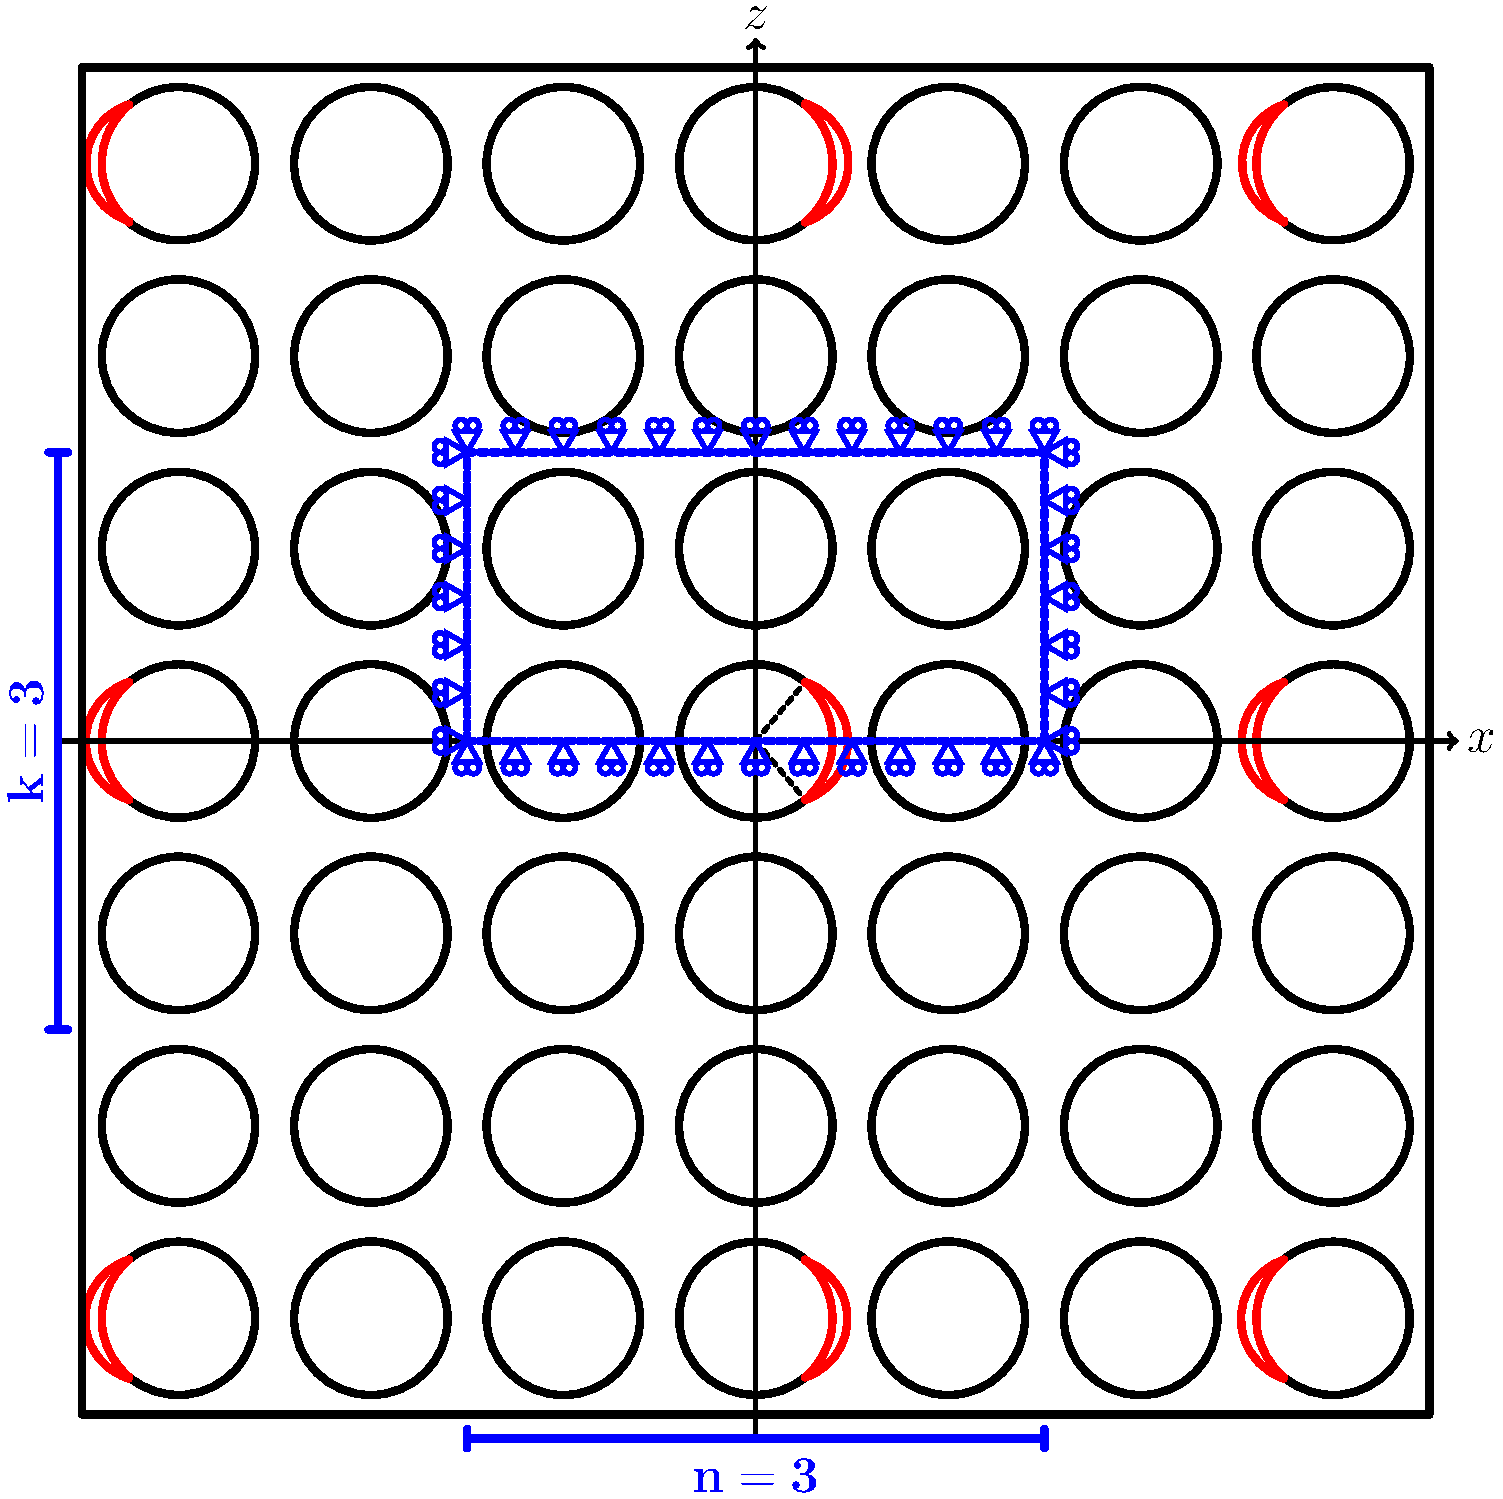
\includegraphics[height=0.225\textheight]{paperD/coupling.pdf}
\caption{Representative Volume Element $n \times k-symm$ of a UD composite with debonds appearing after $n-1$ and after $k-1$ undamaged fibers respectively in the horizontal and vertical direction. In the vertical direction, on fibers belonging to the same ´´column", debonds are located always on the same side.}\label{paperD:fig:coupling-rve}
\end{figure}

The first family has coupling conditions applied to the vertical displacement of the points belonging to the upper side, such that

\begin{equation}
u_{z}\left(x,h\right)=u_{z}^{\nu},
\end{equation}

where $h$ is the height of the RVE and $u_{z}^{\nu}$ is the unknown constant vertical displacement of the upper boundary due to Poisson’s effect, which is evaluated as part of the elastic solution. This condition implies that the element is repeating along the vertical direction, symmetrically with respect to the upper boundary line. It means, in turn, that the next debonded fiber will have a debond on the same side as the preceding one (see Fig.~\ref{paperD:fig:coupling-rve}). We will refer to this set of RVEs as $n \times k-symm$, where $n$ and $k$ are the number of fibers respectively in the RVE’s horizontal and vertical direction.

\begin{figure}[!htb]
\centering
  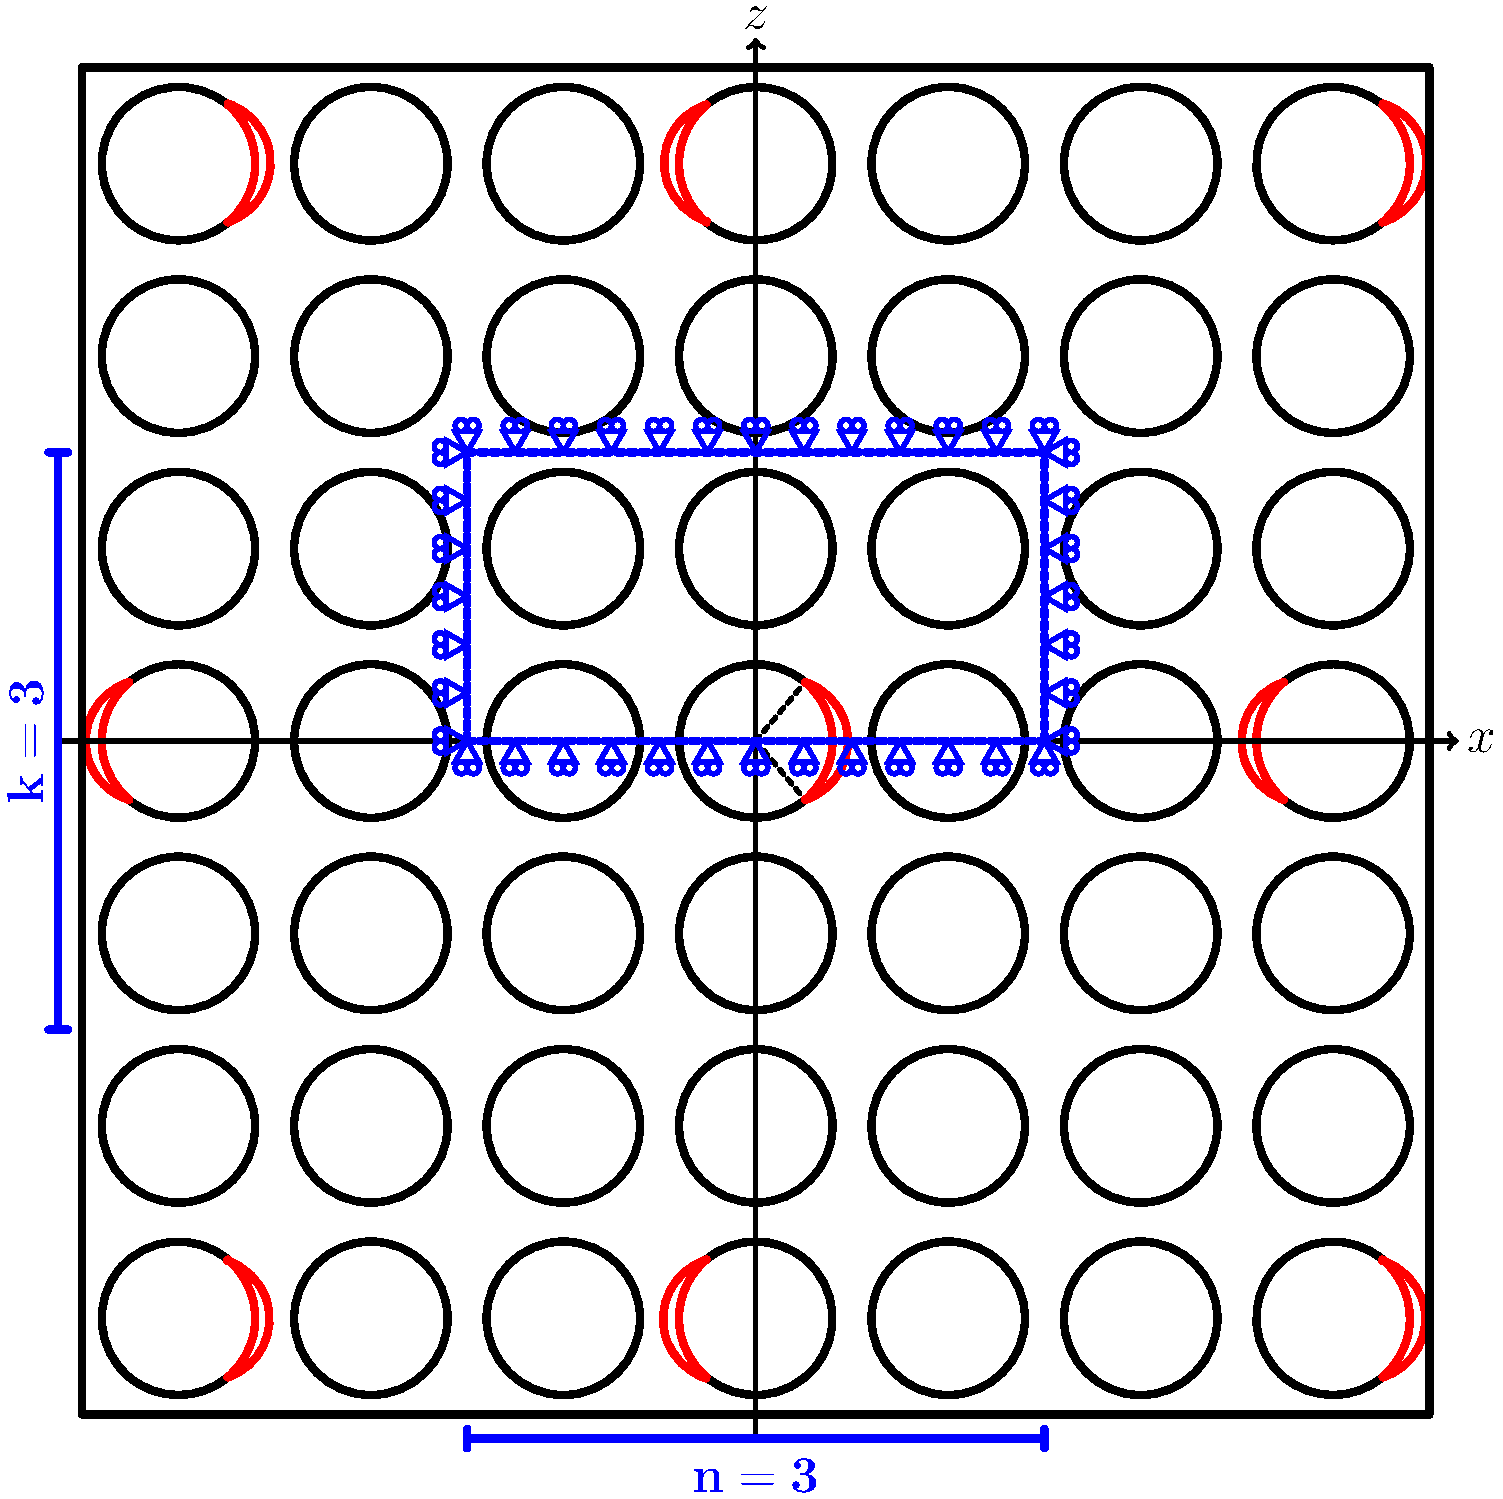
\includegraphics[height=0.225\textheight]{paperD/asymm.pdf}
\caption{Representative Volume Element $n \times k-asymm$ of a UD composite with debonds appearing after $n-1$ and after $k-1$ undamaged fibers respectively in the horizontal and vertical direction. In the vertical direction, on fibers belonging to the same ´´column", debonds are located on the opposite sides of consecutive fibers.}\label{paperD:fig:asymm-rve}
\end{figure}

The second type of RVE has a set of boundary conditions applied to the upper side of the form (see Fig. 3):

\begin{equation}
u_{z}\left(x,h\right)-u_{z}\left(0,h\right)=-\left(u_{z}\left(-x,h\right)-u_{z}\left(0,h\right)\right),
\end{equation}

\begin{equation}
u_{x}\left(x,h\right)=-u_{x}\left(-x,h\right),
\end{equation}

where $h$ is the height of the RVE and $u_{z}\left(0,h\right)$ is the unknown vertical displacement of the upper boundary’s mid-point due to Poisson’s effect, which is evaluated as part of the elastic solution. This condition, an anti-symmetric coupling condition, implies that the element is repeating along the vertical direction, anti-symmetrically with respect to the upper boundary line, i.e. the next debonded fiber will have a debond on the opposite side with respect to the preceding one (see Fig.~\ref{paperD:fig:asymm-rve}). To the authors’ knowledge, this is the first time that this kind of coupling condition is proposed to model the growth of multiple debonds on alternating sides of consecutive fibers along the through-the-thickness direction. We will refer to this set of RVEs as $n \times k-asymm$, where $n$ and $k$ are the number of fibers respectively in the RVE’s horizontal and vertical direction.



%%%%%%%%%%%%%%%%%%%%%%%%%%%%%%%%%%%%%%%%%%%%%%%%%%%%%%%%%%%%%%%%%%%
% 3. RESULTS AND DISCUSSION
%%%%%%%%%%%%%%%%%%%%%%%%%%%%%%%%%%%%%%%%%%%%%%%%%%%%%%%%%%%%%%%%%%%

\section{Finite Element solution}

The length and height of the generic $n \times k-symm$ and $n \times k-asymm$ RVE are respectively defined as

\begin{equation}
l=n\cdot2L\quad h=k\cdot2L,
\end{equation}

where $2L\cdot2L$ is the size of a $1$-fiber unit cell (see Fig. 4) and $L$ is determined by

\begin{equation}
L=\frac{R_{f}}{2}\sqrt{\frac{\pi}{V_{f}}},
\end{equation}

where $R_{f}$ and $V_{f}$ are respectively the fiber radius and volume fraction. The fiber radius is assumed to be always equal to $1\ μm$: within the scope of Linear Elastic Fracture Mechanics (LEFM), the ERR is linearly proportional to the fiber radius, which is representative of the crack size. Thus, the fiber radius represents a scale parameter and a simple multiplication is needed to obtain the ERR for a different value of the fiber radius. The volume fraction is assumed to be homogeneous and equal to $60\%$.

\begin{figure}[!htb]
\centering
  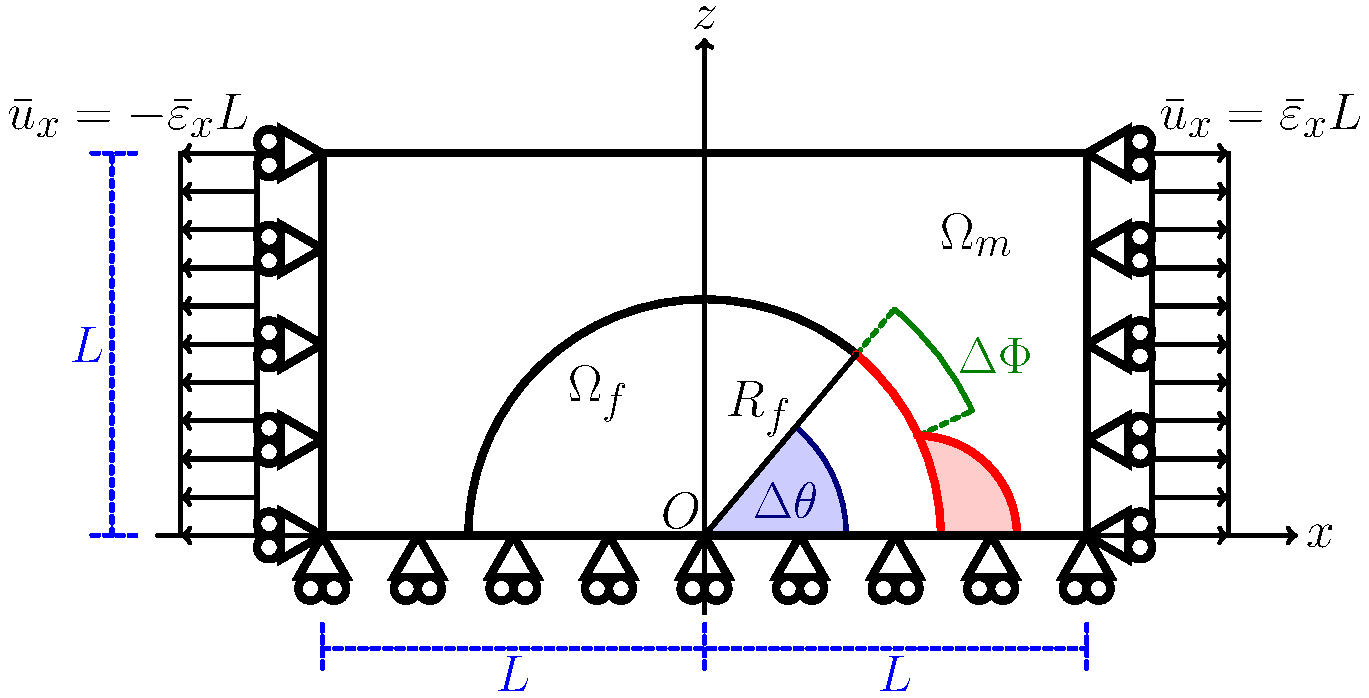
\includegraphics[height=0.225\textheight]{paperD/RUC.pdf}
\caption{Schematic of the model with its main parameters.}\label{paperD:fig:ruc}
\end{figure}
%%%%%%%%%%%%%%%%%%%%%%%%%%%%%%%%%%%%%%%%%%%%%%%%%%%%%%%%%%%%%%%%%%%
% 4. CONCLUSIONS AND OUTLOOK
%%%%%%%%%%%%%%%%%%%%%%%%%%%%%%%%%%%%%%%%%%%%%%%%%%%%%%%%%%%%%%%%%%%

\section{Conclusions}

Different models of Repeating Unit Cell, representing different cross-ply laminates, have been studied in order to investigate the effect of the presence of the $0^{\circ}$ layer and of its thickness on debond Energy Release Rate for interactive and non-interactive debonds. A particular damage state is studied, in which only the central row of fibers of the $90^{\circ}$ ply possesses debonds. The thickness of the $90^{\circ}$ ply is measured in terms of the number of fiber rows in the layer; the $0^{\circ}$ layer is on the other hand modelled as a homogenized material, the thickness of which is a multiple of the $90^{\circ}$ ply thickness. In order to investigate the mechanisms of the debond-$0^{\circ}/90^{\circ}$ interface interaction, Mode I and Mode II ERR of cross-ply RUCs are compared with those of RUCs with equivalent boundary conditions on the upper boundary: free surface; coupling conditions on the vertical displacements; an applied linear distribution of the horizontal displacement; coupling conditions on the vertical displacements superimposed to an applied linear distribution of the horizontal displacement (this last combination represents the most extreme effect of the $0^{\circ}$ layer on debond growth). It has been found that:
\begin{itemize}
\item by forcing the $0^{\circ}/90^{\circ}$ interface to remain approximately straight and controlling the uniformity of the horizontal displacements in the composite (and thus in the $90^{\circ}$ ply), the presence of the $0^{\circ}$ layer causes more homogeneous local (i.e. in the debond neighborhood) strains, reducing the ERR at the debond crack tip;
\item when increasing the thickness of the $0^{\circ}$ layer, the effect of the presence of the $0^{\circ}$ layer on debond ERR remains the same as in the case $t_{0^{\circ}}=t_{90^{\circ}}$;
%\item no difference in ERR is seen when one or more rows of fibers with no damage are present between the debond and the $0^{\circ}/90^{\circ}$ interface, a change is observed only no row of undamaged fibers is present between the debond and the $0^{\circ}/90^{\circ}$ interface;
\item no effect of the $90^{\circ}$ layer thickness, measured in terms of number of fiber rows, is observed; a reduction in ERR takes place only when the thickness is reduced to only one fiber row.
\end{itemize}
The results reported in this article strengthen the claim that the ply-thickness effect does not influence the growth of individual debonds, as previously suggested in the literature~\cite{Saito2012,Herraez2015,Velasco2018, Paris2018}.

%%%%%%%%%%%%%%%%%%%%%%%%%%%%%%%%%%%%%%%%%%%%%%%%%%%%%%%%%%%%%%%%%%%
% ACKNOWLEDGEMENTS
%%%%%%%%%%%%%%%%%%%%%%%%%%%%%%%%%%%%%%%%%%%%%%%%%%%%%%%%%%%%%%%%%%%

\section*{Acknowledgements}

Luca Di Stasio gratefully acknowledges the support of the European School of Materials (EUSMAT) through the DocMASE Doctoral Programme and the European Commission through the Erasmus Mundus Programme.


\section*{References}
\addcontentsline{toc}{section}{References}
\printbibliography[heading=none]
